\subsection{Aplikacja serwerowa}

Do zaimplementowania aplikacji serwerowej wykorzystaliśmy:

\begin{itemize}
  \item język programowania Ruby, versja 2.2.2 \cite{bib:ruby-doc}
  \item Framework Ruby on Rails, versja 4.2.3 \cite{bib:rails-doc}
  \item CoffeScript \cite{bib:coffeescript-doc}
  \item Sass \cite{bib:sass-doc}
  \item Bibliotekę jQuery do języka javaScript \cite{bib:jquery-doc}
  \item Bazę danych SQLlite
\end{itemize}

Wybór padł na technologię Ruby on Rails głównie ze względu na łatwość integracji z REST-owym API, ale ważnymi czynnikami były także: szybkość powstawania aplikacji internetowych w tym frameworku, oraz na obecną popularność na rynku.

\subsection {Instalacja i uruchomienie aplikacji serwerowej}

Aby uruchomić środowisko aplikacji, należy mieć zainstalowany język ruby oraz framework Ruby on Rails, wraz ze wszystkimi potrzebnymi wtyczkami. W systemie Ubutntu, aby to osiągnąć, należy najpierw zainstalować manager wersji Ruby (RVM \cite{bib:rvm-install}). Kiedy mamy to zrobione, należy uruchomić terminal, jprzejść do folderu aplikacji, a następnie zainstalować wersję 2.2.2 języka Ruby oraz odpowiedni komplet gemów.

\begin{lstlisting}
  rvm install 2.2.2
  rvm use 2.2.2@test --create
  gem install bundler
  bundle install
\end{lstlisting}


Po zakończeniu wykonywania powyższych komend, śodowisko aplikacji powinno być zainstalowane. Kolejnym krokiem jest uruchomienie lokalnego serwera aplikacji.

\begin{lstlisting}
  rails s
\end{lstlisting}

Od tej pory aplikacja powinna być dostępna pod adresem \url{http://localhost:3000}, co widać na rysunku \ref{figure:root-page-server},

\begin{figure}[ht]
  \centering
  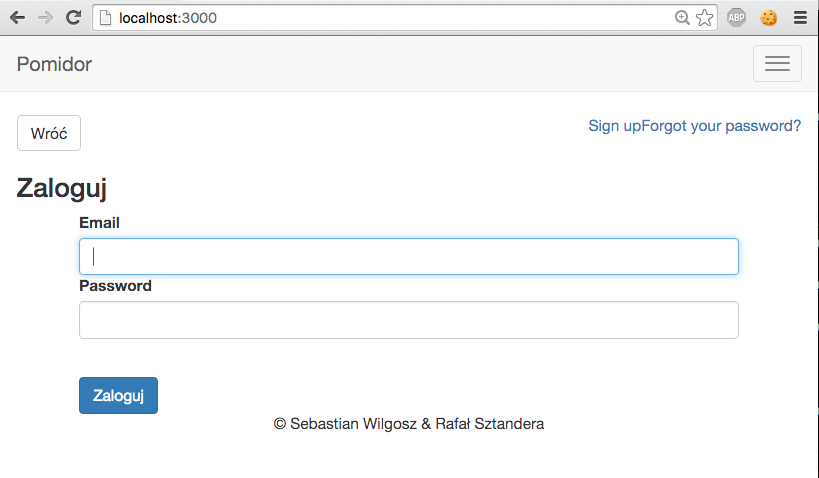
\includegraphics[scale=0.35]{images/root-page-server.png}
  \caption{Widok strony głównej aplikacji}
  \label{figure:root-page-server}
\end{figure}
\FloatBarrier
